\documentclass[aspectratio=169]{beamer}
\usepackage[utf8]{inputenc}
\usepackage{lmodern}
\usepackage{tikz}
\usepackage{hyperref}
\hypersetup{hidelinks}
\usetikzlibrary{positioning,arrows.meta}

\definecolor{accent1}{HTML}{0F766E}
\definecolor{accent2}{HTML}{99F6E4}
\definecolor{accent3}{HTML}{F59E0B}
\definecolor{accent4}{HTML}{134E4A}
\definecolor{paper}{HTML}{F7FEFC}
\definecolor{ink}{HTML}{1F2937}

\newcommand{\PromptCopyBase}{lesson2-3-wrap-up-prompt-cards-copy.html}
\newcommand{\CopyChip}[1]{%
  \href{\PromptCopyBase\##1}{%
    \tikz[baseline=-0.6ex] \node[
      rounded corners=5pt,
      fill=accent2!30,
      draw=accent1,
      line width=0.6pt,
      inner xsep=6pt,
      inner ysep=2pt
    ]{\scriptsize\bfseries Copy};%
  }%
}

\setbeamertemplate{navigation symbols}{}
\setbeamercolor{normal text}{fg=ink,bg=white}
\setbeamercolor{frametitle}{fg=ink,bg=white}
\setbeamertemplate{itemize item}{\color{accent1}$\blacktriangleright$}
\setbeamertemplate{enumerate item}{\color{accent1}\insertenumlabel.}
\setbeameroption{hide notes}

\title{Lesson 2-3: Build, Check, Finish}
\subtitle{MagicSchool AI Project Wrap-Up}
\author{Pine Brook IGNITE}
\date{Spring 2026}

\begin{document}

\begin{frame}[plain]
\begin{tikzpicture}[remember picture,overlay]
\fill[paper] (current page.south west) rectangle (current page.north east);
\fill[accent1!10] (0.35,0.45) rectangle (12.95,7.05);
\draw[line width=7pt, color=accent3] (0.65,6.78) -- (12.65,6.78);
\draw[line width=7pt, color=accent2] (0.65,0.72) -- (12.65,0.72);
\end{tikzpicture}
\vspace{0.75cm}
{\huge\bfseries Lesson 2-3: Build, Check, Finish\par}
\vspace{0.25cm}
{\Large\color{accent4} Today we wrap up the AI project in 4 steps.\par}
\vspace{0.55cm}
\begin{center}
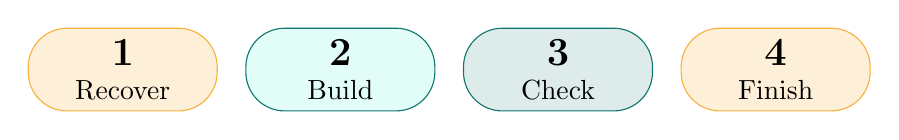
\begin{tikzpicture}[node distance=0.35cm]
\node[rounded corners=14pt, fill=accent3!16, draw=accent3!80, minimum width=2.4cm, minimum height=1.05cm, align=center] (a) {\Large\bfseries 1\\Recover};
\node[rounded corners=14pt, fill=accent2!28, draw=accent1, minimum width=2.4cm, minimum height=1.05cm, align=center, right=of a] (b) {\Large\bfseries 2\\Build};
\node[rounded corners=14pt, fill=accent1!14, draw=accent1, minimum width=2.4cm, minimum height=1.05cm, align=center, right=of b] (c) {\Large\bfseries 3\\Check};
\node[rounded corners=14pt, fill=accent3!16, draw=accent3!80, minimum width=2.4cm, minimum height=1.05cm, align=center, right=of c] (d) {\Large\bfseries 4\\Finish};
\end{tikzpicture}
\end{center}
\vspace{0.35cm}
\begin{block}{Big idea}
\Large AI can help us finish, but we make the choices.
\end{block}
\end{frame}

\begin{frame}[plain]
\frametitle{Today You Need}
\begin{block}{By the end, you should have:}
\begin{itemize}
\Large
\item a topic
\item 3 project parts or slides
\item one AI check
\item one final reflection
\end{itemize}
\end{block}
\vspace{0.25cm}
\begin{center}
\Large Build first. Check second. Finish third.
\end{center}
\end{frame}

\begin{frame}[plain]
\frametitle{Step 1: Recover}
\begin{block}{If you already have a topic and guide}
\Large Go straight to Step 2.
\end{block}
\vspace{0.2cm}
\begin{block}{If you are missing your guide}
\Large \CopyChip{recover}\hspace{0.5em}\texttt{My topic is \_\_\_\_. Help me make a simple project guide with 3 parts. Each part should be short and connected to computer science.}
\end{block}
\end{frame}

\begin{frame}[plain]
\frametitle{Step 2: Build One Slide}
\begin{block}{Use this for each part}
\Large \CopyChip{build}\hspace{0.5em}\texttt{My topic is \_\_\_\_. Part \_\_ of my guide is \_\_\_\_. Give me 3 short bullet notes I can use on one slide. Keep it clear for Grade 4.}
\end{block}
\vspace{0.25cm}
\begin{block}{Build rule}
\Large Use the notes to make your own slide. Do not paste everything without reading.
\end{block}
\end{frame}

\begin{frame}[plain]
\frametitle{Simple Example}
\begin{columns}[T,totalwidth=\textwidth]
\column{0.48\textwidth}
\begin{block}{Topic and guide}
\large
Topic: robots help animals

Part 1: what robots are

Part 2: how robots help

Part 3: why it matters
\end{block}
\column{0.48\textwidth}
\begin{block}{One slide}
\large
Title: How robots help

Robots can use sensors.

Robots can follow code.

Robots can do jobs safely.
\end{block}
\end{columns}
\end{frame}

\begin{frame}[plain]
\frametitle{Step 3: Check Your Project}
\begin{block}{Use this after you build}
\Large \CopyChip{check}\hspace{0.5em}\texttt{My topic is \_\_\_\_. My guide is \_\_\_\_. Here is my project text: \_\_\_\_. Tell me what matches, what is missing, and what I should fix first.}
\end{block}
\vspace{0.25cm}
\begin{block}{Check rule}
\Large Fix one thing first. Keep it simple.
\end{block}
\end{frame}

\begin{frame}[plain]
\frametitle{Step 4: Finish}
\begin{block}{Add your final reflection}
\Large \CopyChip{finish}\hspace{0.5em}\texttt{Help me write a short final reflection. I used AI to \_\_\_\_. I made my own choices by \_\_\_\_. Keep it 2 sentences.}
\end{block}
\vspace{0.25cm}
\begin{block}{Finish rule}
\Large Your reflection should sound like you.
\end{block}
\end{frame}

\begin{frame}[plain]
\frametitle{Before You Turn It In}
\begin{block}{Final checklist}
\begin{itemize}
\Large
\item My topic is clear.
\item I have 3 parts or slides.
\item I checked my project with AI.
\item I fixed one thing.
\item I wrote my reflection.
\end{itemize}
\end{block}
\end{frame}

\begin{frame}[plain]
\frametitle{Exit Ticket}
\begin{block}{Answer before you leave}
\begin{itemize}
\Large
\item What did you finish?
\item What did AI help with?
\item What did you decide yourself?
\item What would you improve next time?
\end{itemize}
\end{block}
\vspace{0.25cm}
\begin{center}
\Large Save your work before you close your Chromebook.
\end{center}
\end{frame}

\end{document}
